\section{zmq-broker}

A message broker prototype was developed to get a feel for how \ngrm\ 
comms services can be built as plugins communicating with messages.
This experiment builds on lessons learned from the previous PMI
investigation, implementing scalable barriers, a key-value service,
and a public interface suitable for linking with applications.

\begin{figure}
\centering
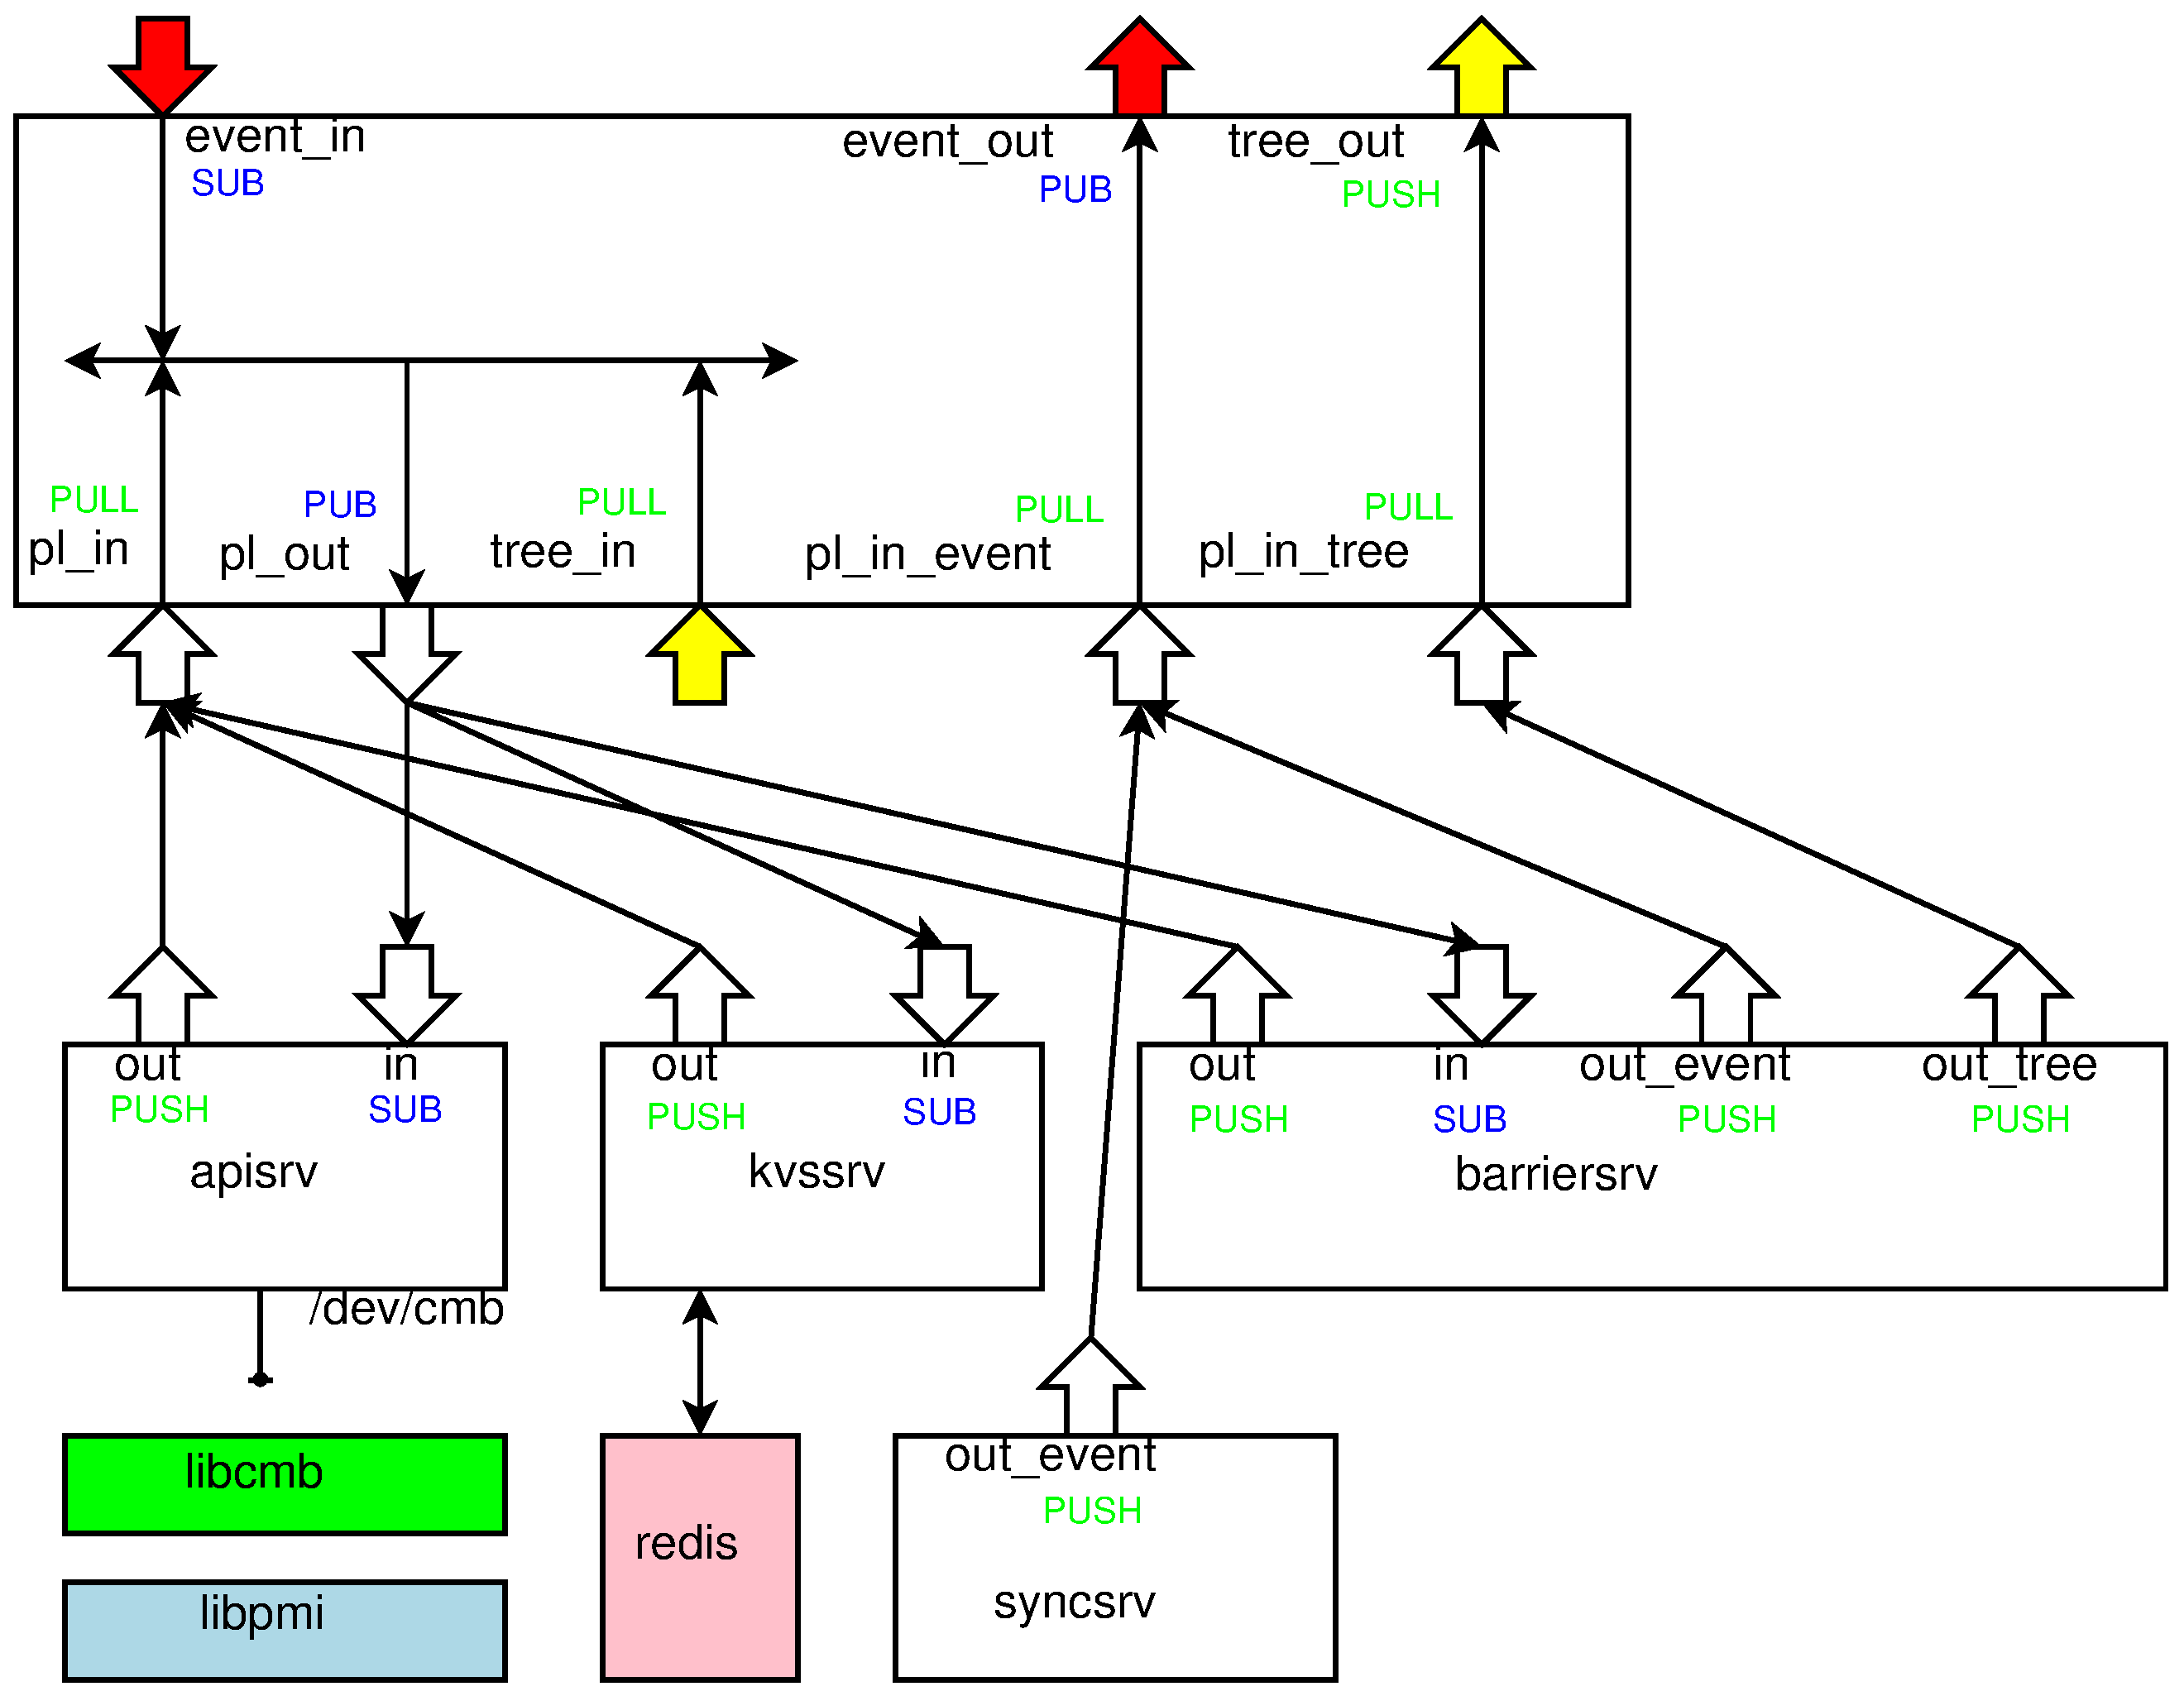
\includegraphics[scale=0.30]{zmq-broker.eps}
\caption{Broker internal architecture.  The cmbd simply routes messages
between \zMQ\ sockets, while plugins (syncsrv, apisrv, kvssrv, barriersrv)
perform specialized services.
Plugins are implemented as threads spawned by the cmbd, and communicate
with the cmbd using {\em inproc} (shared memory) \zMQ\ sockets.
The {\em libcmb} library, which provides the system's public interfaces,
communicates with the apisrv plugin via a UNIX domain socket.}
\label{fig:cmbint}
\end{figure}

\subsection{The Prototype}

\paragraph {Internal Design}
The internal architecture is shown in Figure~\ref{fig:cmbint}.
The cmbd acts as a message router, passing two-part \zMQ\ messages
(Figure~\ref{fig:cmbproto}) between sockets as defined in
Table~\ref{tab:cmbrouting}.
Plugins are implemented as cmbd threads that access well known \zMQ\ sockets.
Public interfaces are exposed by a library which access the CMB through
a UNIX domain socked exposed by the {\em apisrv} plugin.
The public API is depicted in Table~\ref{tab:cmbapi}.

\begin{table}
\centering
\begin{tabular}{|l|l|l|l|}\hline
\textbf{Plugin-sock} & \textbf{CMB-sock} & \textbf{CMB-sock}
					 & \textbf{External} \\
\hline
out (PUSH)		& pl\_in (PULL)	& {\em BUS} & \\
out\_event (PUSH)  & pl\_in\_event (PULL) & event\_out (PUB) & $\rightarrow$ \\
out\_tree (PUSH) & pl\_in\_tree	(PULL) & tree\_out (PUSH) & $\rightarrow$ \\
in (SUB)	& pl\_out (PUB)	& {\em BUS}     & \\
\hline
		& {\em BUS}	& event\_in (SUB) & $\leftarrow$ \\
		& {\em BUS}	& tree\_in (PULL) & $\leftarrow$ \\
\hline
\end{tabular}
\caption{The cmbd internal routing table.}
\label{tab:cmbrouting}
\end{table}

\begin{figure}
\centering
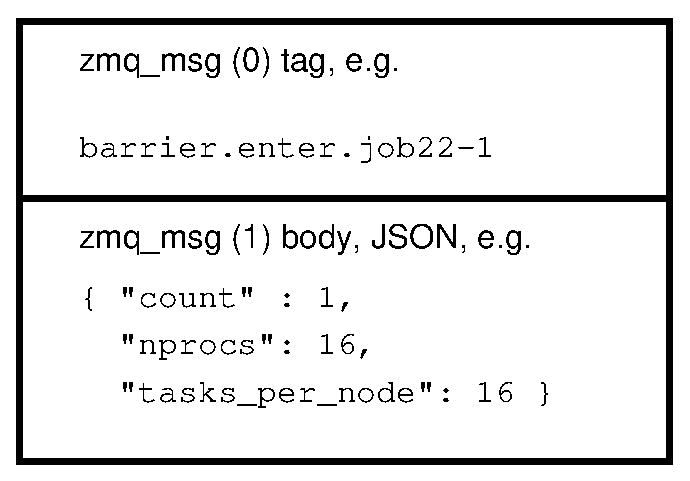
\includegraphics[scale=0.4]{zmq-broker-proto.eps}
\caption{Message protocol.  Messages consist of two \zMQ\ message parts.
The first part is a {\em tag} formatted as a zmQ string suitable for
use as a subscription tag on PUB-SUB sockets, and which is used to identify
the recipient(s).
The second part is JSON formatted as a \zMQ\ string.}
\label{fig:cmbproto}
\end{figure}

\paragraph {External Design}
The cmbd implements the reduction network and event service described
in the \ngrm\ comms design.

\begin{figure}
\centering
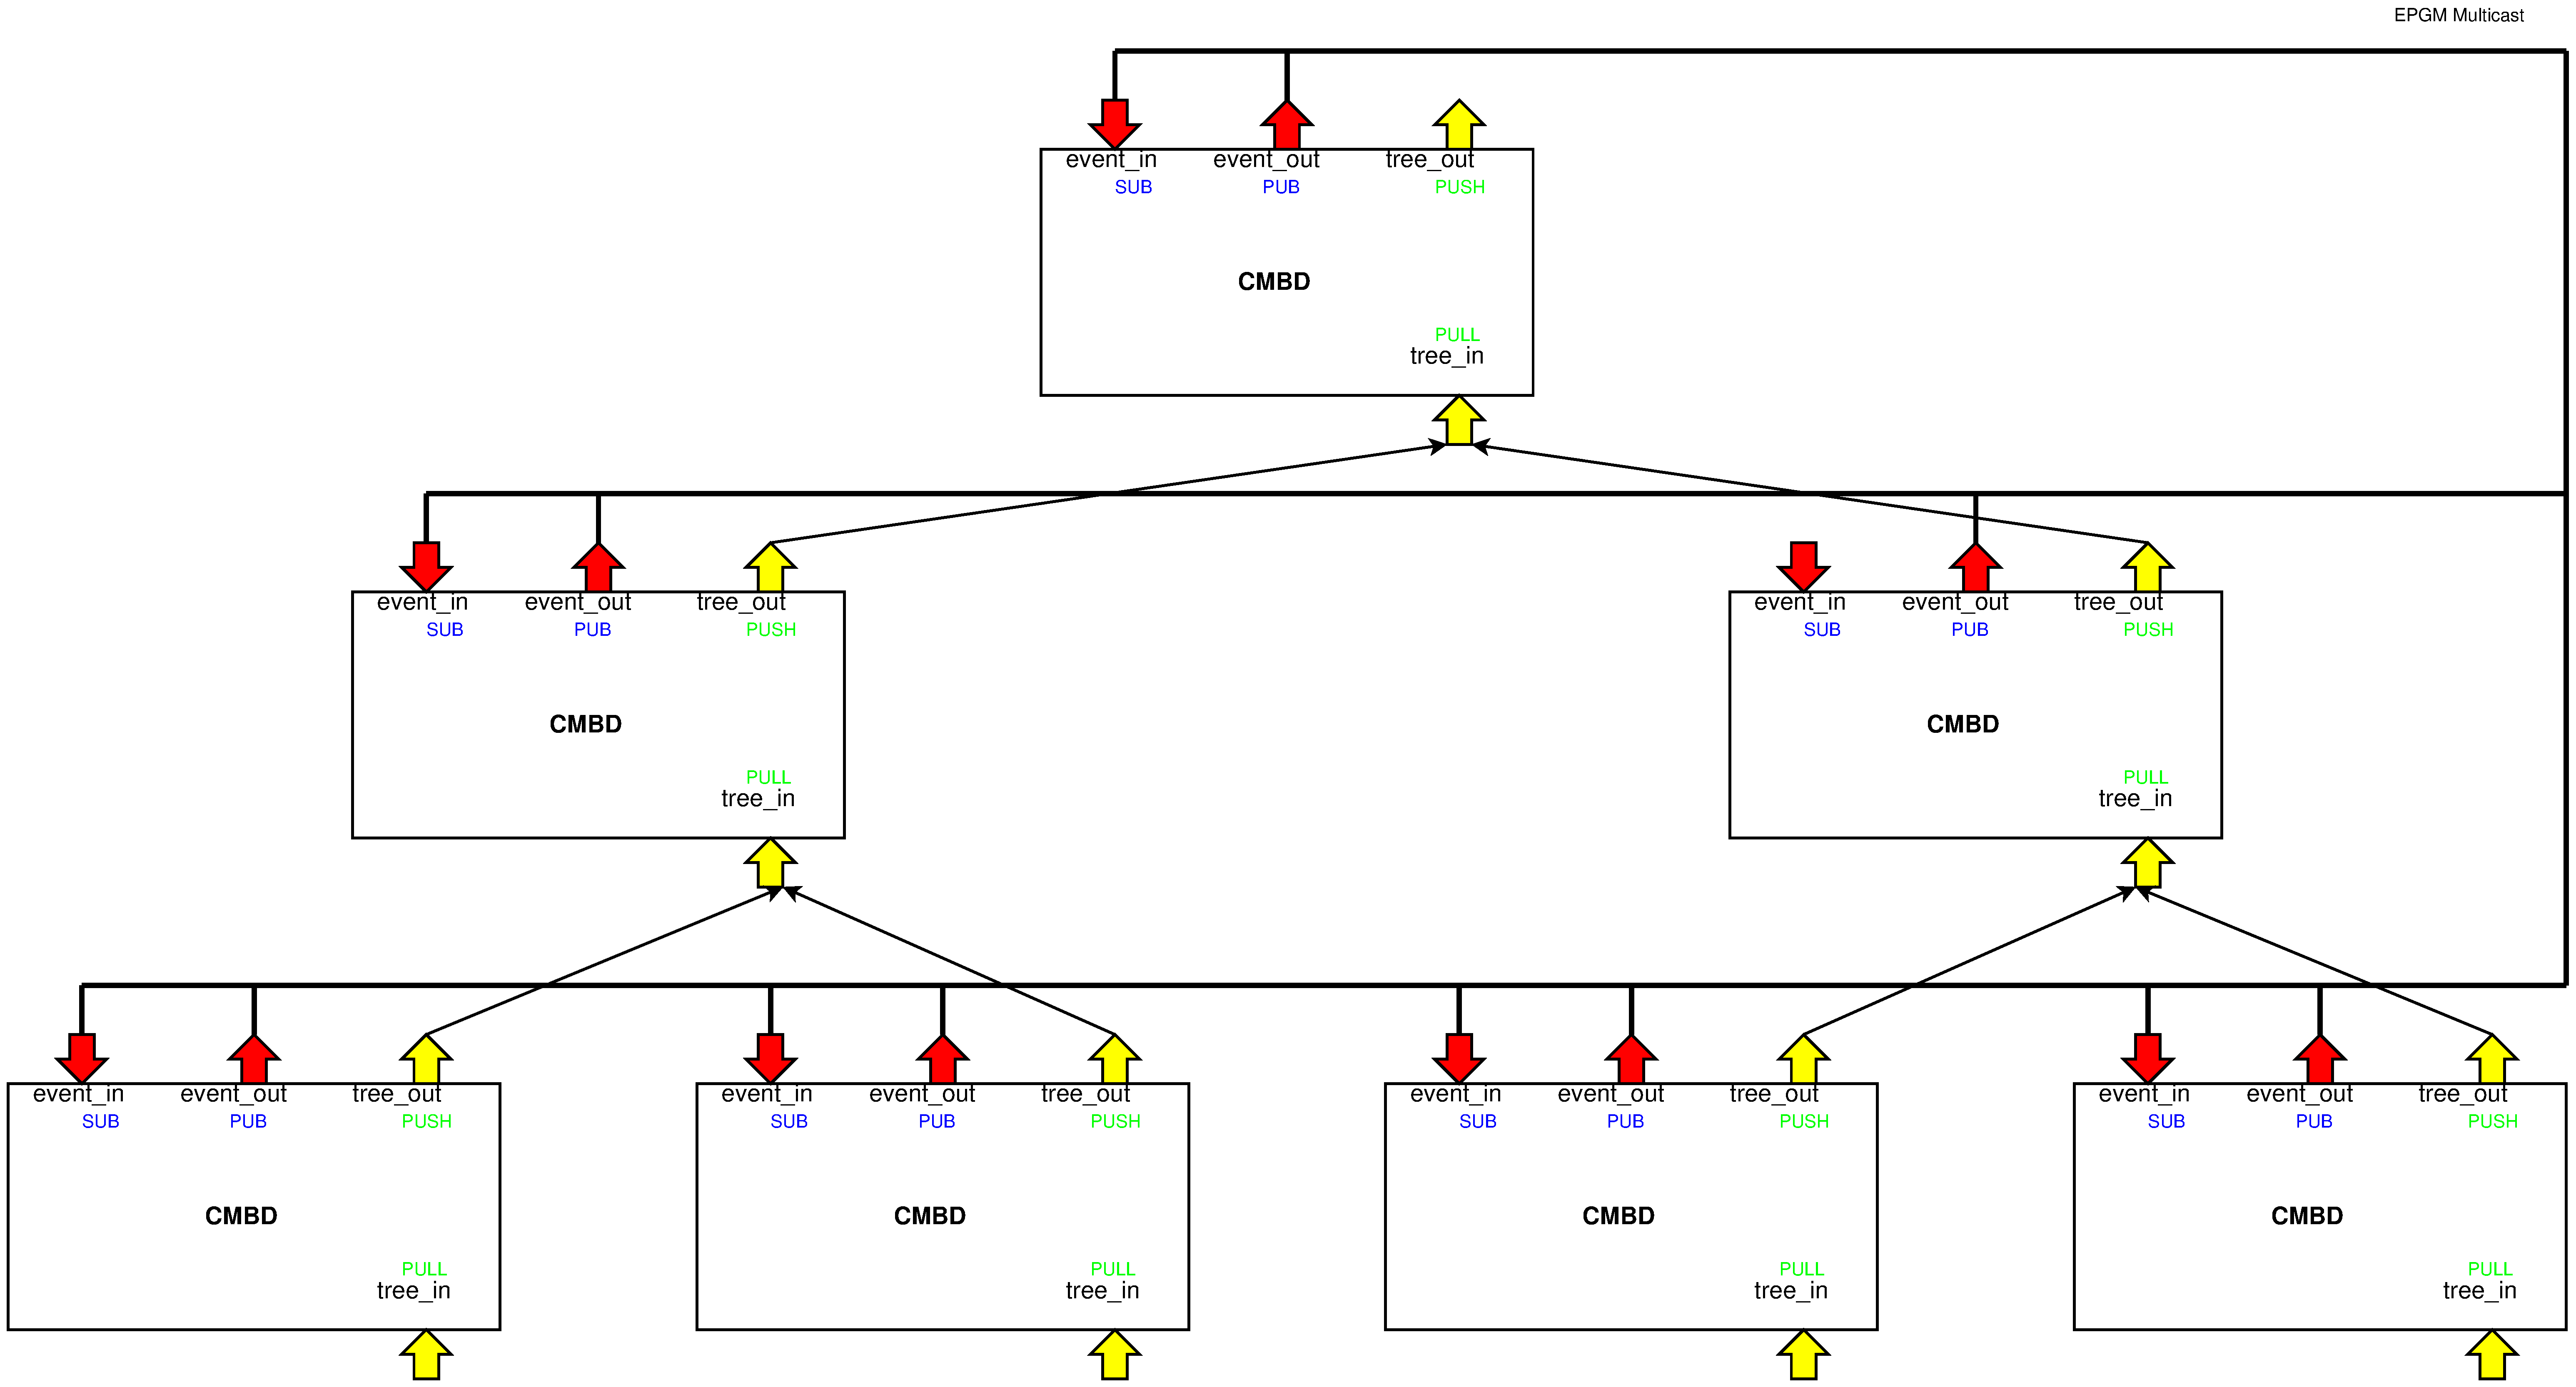
\includegraphics[scale=0.15]{zmq-broker-tree.eps}
\caption{Broker external architecture.}
\label{fig:cmbext}
\end{figure}


\begin{table}
\centering
\begin{tabular}{|p{0.7cm}p{5cm}|p{9cm}|}\hline
\multicolumn{2}{|l|}{\textbf{Function}}
  & \textbf{Description} \\
\hline
{\tt cmb\_t} & {\tt cmb\_init (void)}
  & Create a {\em cmb\_t} context for communicating with the broker.\\
{\tt void} & {\tt cmb\_fini (cmb\_t c)}
  & Destroy a {\em cmb\_t} context.\\
\hline
{\tt int} & {\tt cmb\_ping (cmb\_t c, int seq, int padding)}
  & Send a ping message to the broker's internal bus and wait for it
    to be echoed back.  {\em padding} bytes of payload will be added to
    the message.
    On success, returns $0$; on failure, returns $-1$ with errno set.\\
\hline
{\tt int} & {\tt cmb\_snoop (cmb\_t c, char {*sub})}
  & Print all messages on the broker's internal bus whose tags match the
    subscription string {\em sub}.  The empty string matches all messages.
    On success, does not return; on failure, returns $-1$ with errno set.\\
\hline
{\tt int}
  & {\tt cmb\_barrier (cmb\_t c, char {*name}, int nprocs,
                       int procs\_per\_node)}
  & Execute barrier {\em name}.  The call blocks until {\em nprocs}
    processes have entered the barrier.  If $procs\_per\_node < nprocs$
    then the tree network is used to resolve the barrier.
    On success, returns $0$; on failure, returns $-1$ with errno set.\\
\hline
{\tt int}
  & {\tt cmb\_sync (cmb\_t c)}
  & Block until {\em event.sched.trigger} is received.  This event is
    a job-wide, periodic multicast signal used to synchronize system noise.
    By default it is sent out every $10s$.
    On success, returns $0$; on failure, returns $-1$ with errno set.\\
\hline
{\tt int}
  & {\tt cmb\_kvs\_put (cmb\_t c, char {*key}, char {*val})}
  & Set {\em key} to {\em val} in the job-wide key-value store.
    If the key already has a value, it is overwritten.
    Errors resulting from the actual KVS transaction are not reported
    until the next {\em cmb\_kvs\_commit} call.
    On success, returns $0$; on failure, returns $-1$ with errno set.\\
{\tt {char*}}
  & {\tt cmb\_kvs\_get (cmb\_t c, char {*key})}
  & Retrieve the value of {\em key} from the job-wide key-value store.
    On success, returns a copy of value which the caller must free;
    on failure, returns NULL with errno set.\\
{\tt int}
  & {\tt cmb\_kvs\_commit (cmb\_t c, int *errcount, int *putcount)}
  & Block until the job-wide key-value store has completed all transactions
    originating on the local node.  {\em putcount} will contain the number
    of {\em cmb\_kvs\_put} calls executed by this context since the last commit.
    {\em errcount} will contian the number of failed puts since the last commit.
    On success, returns $0$; on failure, returns $-1$ with errno set.\\
\hline
\end{tabular}
\caption{Public interfaces exported by the broker.  Users would
{\tt \#include "cmb.h"} and link {\tt -lcmb}.  {\em libcmb} utilizes
a UNIX domain socket exported by the {\em apisrv} plugin to implement
a very lightweight interface suitable for linking with applications such
as MPI runtimes (\zMQ\ is too heavyweight to be used directly by applications.)}
\label{tab:cmbapi}
\end{table}


